\documentclass[final,5p,twocolumn,number,nopreprintline]{elsarticle}

\usepackage{amsmath,amssymb,amsfonts}
\usepackage{newtxtext,newtxmath}
\usepackage{algorithm}
\usepackage{algpseudocode}
\usepackage{booktabs}
\usepackage{graphicx}
\usepackage{multirow}
\usepackage{array}
\usepackage{tabularx}
\usepackage{dblfloatfix}
\usepackage{url}
\usepackage{xcolor}
\usepackage[colorlinks=true,linkcolor=blue,citecolor=blue,urlcolor=blue]{hyperref}
\newcommand{\rev}[1]{{\color{blue}#1}}
\newenvironment{revblock}{\begingroup\color{blue}}{\endgroup}
\journal{Transportation Research Part E: Logistics and Transportation Review}
\bibliographystyle{elsarticle-num}
\biboptions{numbers,sort&compress}
\setlength{\bibsep}{0pt plus 0.3ex}
\renewcommand{\bibfont}{\small}
\emergencystretch=2em

\begin{document}

\begin{frontmatter}

\title{Energy-aware vehicle--UAV cooperative scheduling for transmission line inspection with probabilistic energy prediction}

\author[inst1]{Author names withheld for review}
\affiliation[inst1]{organization={School of Management Science and Engineering}, city={--}, country={China}}

\begin{abstract}
Large-scale transmission-line inspection increasingly relies on coordinated ground vehicles and unmanned aerial vehicles, but routing decisions remain sensitive to uncertain UAV endurance, heterogeneous tower priorities and sparse feasible stopping locations. This paper formulates transmission-line inspection as an uncertainty-aware risk-value vehicle--UAV scheduling problem. \rev{The proposed framework combines same-stop multi-tower sortie patterns, a physics-informed residual energy surrogate, chance-constrained sortie screening, risk-value task prioritization, adaptive large-neighborhood search and metric-aware final portfolio selection.} Computational experiments cover small reference instances, medium and large instances from 30 to 500 towers, energy-prediction accuracy, ablation tests, candidate-stop screening, sensitivity analysis, GIS-grounded cases and stress scenarios. \rev{Relative to fixed ALNS, the proposed method reduces mean risk-weighted completion time by 43.1\% on the 100-tower benchmark and 42.0\% on the 500-tower benchmark; it also removes residual infeasible sorties on the 100-tower benchmark and increases top-risk coverage by 76.0 percentage points in the 200-tower corridor case.}
\end{abstract}

\begin{keyword}
\rev{Vehicle--UAV scheduling \sep transmission line inspection \sep adaptive large neighborhood search \sep probabilistic energy surrogate \sep mixed-integer linear programming \sep same-stop sortie patterns}
\end{keyword}

\end{frontmatter}

\noindent{\small \rev{Revision note: blue text marks passages revised for the same-stop multi-tower sortie assumption, operator visualization, terminology consistency and academic-language cleanup.}}
\vspace{0.8em}

\section{Introduction}
\label{sec:introduction}

Drone-assisted routing has developed from stylized truck--drone delivery into richer air--ground logistics systems involving energy supply, no-fly zones, multimodal operations, automatic heuristic design and synchronized truck--drone fleets \cite{murray2015flying,dorling2017vehicle,otto2018survey,kim2026bidirectional,liu2026evtol,zhang2026airground,shi2026llm,yang2025integrated}. Transmission line inspection is a closely related but operationally distinct setting, where UAVs are increasingly used for autonomous navigation, visual inspection, lidar sensing and defect recognition \cite{hui2019monocular,li2021uavtransmission,nguyen2018visionreview,liu2021uavlidar,zhang2020visualinspection}. A ground vehicle can carry multiple UAVs along road-accessible stops, launch UAVs to inspect nearby towers, wait for recovery and continue along the corridor. Compared with parcel delivery, inspection tasks have corridor geometry, heterogeneous defect risk, payload-dependent sensing time and stronger energy-safety requirements.

\rev{This study is organized around three methodological components. A compact MILP provides small-instance reference checks, a residual energy surrogate supplies uncertainty-aware sortie parameters, and an ALNS solver scales the scheduling layer to medium and large inspection corridors. The experiment design follows the same logic through small-instance validation, algorithm comparison, energy-prediction assessment, ablation analysis and GIS-grounded case studies.}

The scientific issue is that fixed endurance assumptions can make scheduling conclusions fragile. Drone energy is affected by flight distance, payload, wind, temperature, hovering and sensing time \cite{stolaroff2018energy,zhang2021energyconsumption,aiello2021energy,chiang2019sustainability,cokyasar2023regional}. A physics-informed residual energy surrogate can encode the physical energy component, but a point prediction alone is not enough for safe dispatch. Therefore, this paper studies both point energy ALNS and a probabilistic, risk-value-aware variant that uses a q95 energy margin when screening sorties. The intended contribution is not merely another ALNS implementation, but an evidence chain linking physics-aware prediction, compact MILP reference validation and scalable vehicle--UAV inspection scheduling.

The contributions are:
\begin{enumerate}
    \item \rev{A vehicle--UAV transmission-line inspection model is built with same-stop multi-tower sortie patterns, repeated UAV dispatch at a stop and energy-surrogate flight time, inspection time, energy and endurance parameters.}
    \item A compact MILP reference model is solved with HiGHS on proposal-defined S-scale instances as a bounded S-scale sanity check.
    \item \rev{An energy-surrogate ALNS is developed with clustering-based pre-screening, five destroy operators, four named repair operators, simulated-annealing acceptance, adaptive operator weights and a metric-aware final candidate portfolio.}
    \item \rev{A computational experiment suite is executed on S/M/L instances from 10 to 500 towers, including baseline comparison, energy prediction accuracy, ablation, candidate-stop screening, statistical testing and GIS-grounded case studies.}
\end{enumerate}

\section{Related work}
\label{sec:related}

The flying sidekick traveling salesman problem established a canonical truck--drone routing model \cite{murray2015flying}. Subsequent studies developed optimization models for the traveling salesman problem with drone \cite{agatz2018tspdrone,poikonen2019branch,roberti2021exact}, vehicle routing problems with drones \cite{poikonen2017extended,wang2017worstcase,wang2019vrpd}, and drone-delivery variants with energy, multi-trip and public-transport recharging assumptions \cite{dorling2017vehicle,moadab2022drone,asoc2023recharging}. Matheuristics and ALNS methods are common because exact synchronization models become difficult at scale \cite{schermer2019matheuristic,sacramento2019alns}. Reviews show that truck--drone routing has expanded into a broad family of synchronization, energy and fleet-planning problems \cite{otto2018survey,macrina2020review,liang2022survey}.

Recent Transportation Research Part E studies further show how air--ground logistics models are expanding. Kim et al. \cite{kim2026bidirectional} study bidirectional energy supply logistics with aerial and ground vehicles. Liu et al. \cite{liu2026evtol} optimize an eVTOL-and-drone system in continuous space with no-fly zones. Zhang et al. \cite{zhang2026airground} integrate drones, aircraft and ground vehicles for joint passenger and parcel mobility. Shi and Zhen \cite{shi2026llm} use LLM-based automatic heuristic design for vehicle-drone routing, and Yang and Li \cite{yang2025integrated} integrate order splitting, allocation and synchronized truck--drone delivery. Same-day and heterogeneous-fleet studies further show that dynamic dispatch and learning-based policies are relevant when vehicle and UAV resources interact \cite{ulmer2018sameday,chen2022deepq}. \rev{Together, these studies motivate an inspection model that specifies the operational interface between vehicles and UAVs, scales beyond exact synchronization models and reports a broad computational protocol.}

Energy feasibility is a second line of literature. Delivery-drone energy has been evaluated from life-cycle, power-model and routing-optimization perspectives \cite{stolaroff2018energy,zhang2021energyconsumption,aiello2021energy,chiang2019sustainability,cokyasar2023regional}. Electric-vehicle routing also provides useful analogues for endurance limits, recharging choices and time-window coupling \cite{schneider2014evrptw,desaulniers2016evrp}. For transmission-line inspection, the operational setting differs from parcel delivery because the tasks follow a corridor, the inspection value is risk-dependent, and UAVs must capture reliable condition data. Existing work covers autonomous transmission-line navigation, power-line inspection surveys, lidar-assisted inspection and deep-learning-based component detection \cite{hui2019monocular,ahmed2024powerline,li2021uavtransmission,nguyen2018visionreview,liu2021uavlidar,zhang2020visualinspection,li2025deeppowerline}.

ALNS remains a strong framework for routing variants because destroy and repair operators can absorb heterogeneous constraints \cite{ropke2006alns,sacramento2019alns}; simulated-annealing acceptance is a standard way to escape local minima \cite{kirkpatrick1983annealing}. For this paper, the important extension is the integration of a physical surrogate and decision uncertainty. Physics-informed neural networks provide a way to embed residuals from physical equations into learned models \cite{raissi2019pinn,karniadakis2021piml,lu2021deepxde,cuomo2022pinnreview}, and Bayesian energy surrogates show how noisy observations can be represented probabilistically \cite{yang2021bpinn}. The chance-style q95 feasibility filter used here is also consistent with robust decision-making principles for uncertain optimization \cite{bertsimas2004robustness}. We use these ideas to update UAV energy, endurance and service-time parameters before and during ALNS search.

\section{Problem description and MILP model}
\label{sec:model}

\begin{revblock}
Let $\mathcal{T}$ be the set of towers, $\mathcal{P}$ the candidate vehicle stops, $\mathcal{V}$ the ground vehicles and $\mathcal{D}_v$ the UAVs carried by vehicle $v$. Each tower $i\in\mathcal{T}$ has coordinates, service time $s_i$, payload $q_i$, defect-risk score $r_i$ and inspection value $\nu_i$. The ground vehicle travels over road arcs between stops, while a UAV is launched from a stop $s$ to execute a same-stop sortie pattern $k\in\mathcal{K}_s$ that may inspect one or more nearby towers before returning to $s$. After recovery, the same UAV can be assigned another sortie pattern from the same visited stop, and several UAVs carried by the vehicle can work in parallel while the vehicle waits.
\end{revblock}

\rev{Figure~\ref{fig:network-construction} gives the graph-based view used to build the inspection network. Candidate vehicle stops and towers form a heterogeneous node set, road arcs connect vehicle stops, and feasible support edges define the same-stop UAV sortie patterns retained after q95 energy screening.}

\begin{figure*}[t]
\centering
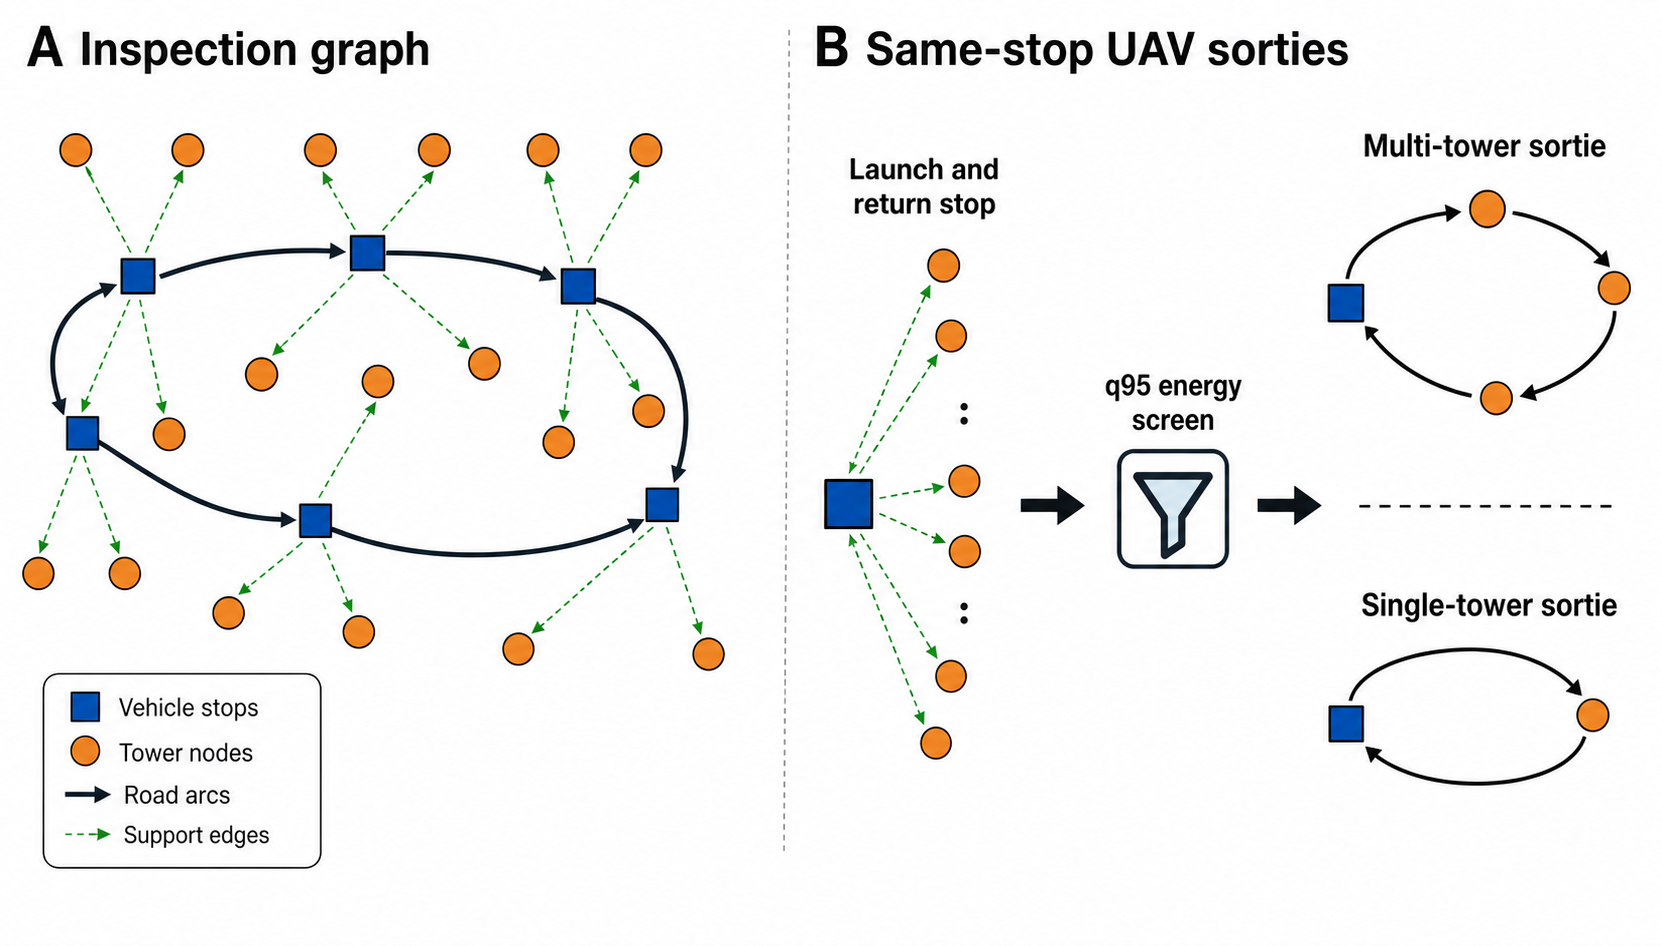
\includegraphics[width=\textwidth]{figures/Fig0_network_construction_ai.png}
\caption{\rev{Graph-based representation of the vehicle--UAV inspection network. Panel A shows the candidate inspection graph with vehicle stops, tower nodes, road arcs and feasible stop--tower support edges. Panel B highlights same-stop UAV sortie patterns, including a multi-tower sortie that starts from a vehicle stop, visits multiple towers and returns to the same stop under the q95 energy feasibility screen.}}
\label{fig:network-construction}
\end{figure*}

\begin{table*}[t]
\centering
\caption{Main notation used in the vehicle--UAV inspection model.}
\label{tab:notation}
{\scriptsize
\setlength{\tabcolsep}{3pt}
\renewcommand{\arraystretch}{0.95}
\begin{tabularx}{\textwidth}{@{}llX@{}}
\toprule
Category & Symbol & Meaning \\
\midrule
Sets & $\mathcal{T}$, $\mathcal{P}$, $\mathcal{V}$, $\mathcal{D}_v$, $\mathcal{K}_s$ & \rev{Towers, candidate vehicle stops, ground vehicles, UAVs carried by vehicle $v$ and feasible same-stop multi-tower sortie patterns launched from stop $s$.} \\
Tower attributes & $s_i$, $q_i$, $r_i$, $\nu_i$ & Inspection service time, sensing payload, defect-risk score and inspection value of tower $i$. \\
Routing decisions & $x^v_{ij}$, $z_s^v$, $y^d_{sk}$ & \rev{Binary decision for vehicle arc $(i,j)$, stop visit and assignment of same-stop sortie pattern $k$ at stop $s$ to UAV $d$. Multiple selected patterns may be assigned to the same recovered UAV at a visited stop.} \\
Timing variables & $t_i^v$, $w_i^v$, $L_s^d$, $\hat\tau^d_{sk}$ & \rev{Vehicle arrival time, vehicle waiting time, sequential workload assigned to UAV $d$ at stop $s$ and predicted UAV sortie duration.} \\
Energy prediction & $\hat E_i$, $Q^d_{sk}$, $\mu_E(x_{sk})$, $\sigma_E(x_{sk})$ & \rev{Tower-level predicted energy, q95 pattern energy, predictive mean and predictive standard deviation from the energy-surrogate interface.} \\
Endurance and safety & $\hat B_d$, $\rho$, $z_\epsilon$ & Predicted UAV endurance, battery reserve ratio and quantile coefficient for chance-style screening. \\
Objective terms & $C_{\max}$, $C_{travel}$, $C^{energy surrogate}_{energy}$ & Completion time, vehicle-travel cost and surrogate-predicted UAV energy term. \\
\bottomrule
\end{tabularx}
}
\end{table*}

Following the proposal, UAV energy contains hovering, level-flight, sensor and wind-disturbance terms:
\begin{equation}
E_i=P^{\mathrm{hover}}t_i^{\mathrm{hover}}
\,+\,\left(a v^3+\frac{m g}{2\eta v}\right)t_i^{\mathrm{flight}}
\,+\,P^{\mathrm{sensor}}s_i
\,+\,C^{\mathrm{wind}}d_i^{\mathrm{air}} .
\label{eq:energy}
\end{equation}
The energy surrogate maps battery state, UAV weight, wind speed/direction, temperature, flight distance and inspection workload to predicted energy $\hat E_i$, flight time $\hat t^{\mathrm{air}}_i$, service time $\hat s_i$ and endurance $\hat B_d$.

The proposal's weighted objective is written as
\begin{equation}
\min \; \alpha C_{\max}+\beta C_{\mathrm{travel}}+\gamma C_{\mathrm{energy}}^{\mathrm{energy surrogate}},
\label{eq:objective}
\end{equation}
where
\begin{equation}
C_{\mathrm{travel}}=\sum_{v\in\mathcal{V}}\sum_{i,j\in\mathcal{P}} d^{\mathrm{road}}_{ij}x^v_{ij},
\qquad
C_{\mathrm{energy}}^{\mathrm{energy surrogate}}=\sum_{d,s,k}\hat E^d_{sk}y^d_{sk}.
\end{equation}
Let $\mathcal{D}=\cup_v\mathcal{D}_v$, let $\mathcal{P}_0=\mathcal{P}\cup\{0\}$ include the depot, and let $\delta_{ik}=1$ if tower $i$ is included in sortie pattern $k$. Each tower must be covered exactly once:
\begin{equation}
\sum_{v\in\mathcal{V}}\sum_{d\in\mathcal{D}_v}\sum_{s\in\mathcal{P}}\sum_{k\in\mathcal{K}_s}\delta_{ik}y^d_{sk}=1,\qquad \forall i\in\mathcal{T}.
\label{eq:tower-coverage}
\end{equation}
Vehicle routes must form balanced stop visits with one depot departure and one depot return for each active ground vehicle:
\begin{align}
\sum_{j\in\mathcal{P}_0:j\ne s}x^v_{sj} &= z_s^v,&
\sum_{i\in\mathcal{P}_0:i\ne s}x^v_{is} &= z_s^v,\qquad &&\forall s\in\mathcal{P},v\in\mathcal{V},\notag\\
\sum_{j\in\mathcal{P}}x^v_{0j} &= 1,&
\sum_{i\in\mathcal{P}}x^v_{i0} &= 1,\qquad &&\forall v\in\mathcal{V}.
\label{eq:vehicle-flow}
\end{align}
\begin{revblock}
Sortie activation links every selected sortie pattern to a visited vehicle stop without imposing a one-sortie-per-UAV limit:
\begin{equation}
y^d_{sk} \leq z_s^v,\qquad \forall v\in\mathcal{V}, d\in\mathcal{D}_v, s\in\mathcal{P}, k\in\mathcal{K}_s.
\label{eq:sortie-activation}
\end{equation}
The q95 energy feasibility constraint is imposed on the complete same-stop pattern rather than on a single tower:
\begin{equation}
Q^d_{sk} y^d_{sk} \leq \hat B_d(1-\rho),\qquad \forall v\in\mathcal{V}, d\in\mathcal{D}_v, s\in\mathcal{P}, k\in\mathcal{K}_s.
\label{eq:endurance}
\end{equation}
Sequential reuse of a recovered UAV at the same stop is represented by the UAV-specific stop workload
\begin{equation}
L_s^d=\sum_{k\in\mathcal{K}_s}\hat\tau^d_{sk}y^d_{sk},\qquad \forall v\in\mathcal{V}, d\in\mathcal{D}_v, s\in\mathcal{P}.
\label{eq:uav-chain}
\end{equation}
The vehicle can dispatch multiple UAVs in parallel at stop $s$, but it cannot depart until every assigned UAV chain has returned:
\begin{align}
t_j^v &\geq t_i^v+w_i^v+\frac{d^{\mathrm{road}}_{ij}}{v^{\mathrm{car}}}-M(1-x^v_{ij}),
\qquad \forall i,j\in\mathcal{P}_0,v\in\mathcal{V},
\label{eq:time-propagation}\\
w_s^v &\geq L_s^d,\qquad \forall v\in\mathcal{V},d\in\mathcal{D}_v,s\in\mathcal{P}.
\label{eq:launch-recovery-sync}
\end{align}
\end{revblock}

\section{energy-surrogate ALNS}
\label{sec:algorithm}

The algorithm follows the three-stage design in the proposal. First, tower coordinates are partitioned by corridor-aware clustering and candidate same-stop sortie candidates are pre-screened by the energy-surrogate endurance estimate. Second, S-scale instances are solved by a compact MILP reference model to provide bounded comparison points. Third, medium and large instances are solved with energy ALNS. \rev{The full probabilistic variant reports the best schedule from a constant-size final portfolio containing the adaptive ALNS search order, a point-energy local order, a UQ-energy local order and a risk-value order. Portfolio selection is lexicographic in infeasible-sortie count, risk-weighted completion time and makespan, aligning the algorithmic final-selection step with the manuscript evaluation metric.}

\begin{table*}[t]
\centering
\caption{Destroy and repair operators in the implemented energy ALNS.}
\label{tab:operators}
\footnotesize
\setlength{\tabcolsep}{4pt}
\renewcommand{\arraystretch}{1.12}
\begin{tabularx}{\textwidth}{@{}p{0.15\textwidth}p{0.30\textwidth}X@{}}
\toprule
Pool & Operators & Search role \\
\midrule
Destroy & Random, worst-energy, Shaw related, path-segment and UAV-chain removals & Diversifies the incumbent, targets high-q95-energy towers, reopens spatially related corridor segments and removes contiguous UAV task chains when synchronization or workload patterns are poor. \\
Repair & Greedy, regret-$k$, energy-minimum and synchronization-aware insertions & Rebuilds feasible schedules by combining risk-value priority, insertion regret, cached q95 energy feasibility and segment workload balancing. \\
\bottomrule
\end{tabularx}
\end{table*}

\rev{Figure~\ref{fig:operator-mechanism} visualizes the destroy--repair operator mechanism used by the ALNS search. The destroy step releases a subset of tasks from the incumbent schedule, the repair step reinserts them with risk-value and q95 feasibility information, and the acceptance step updates the incumbent and operator weights.}

\begin{figure*}[t]
\centering
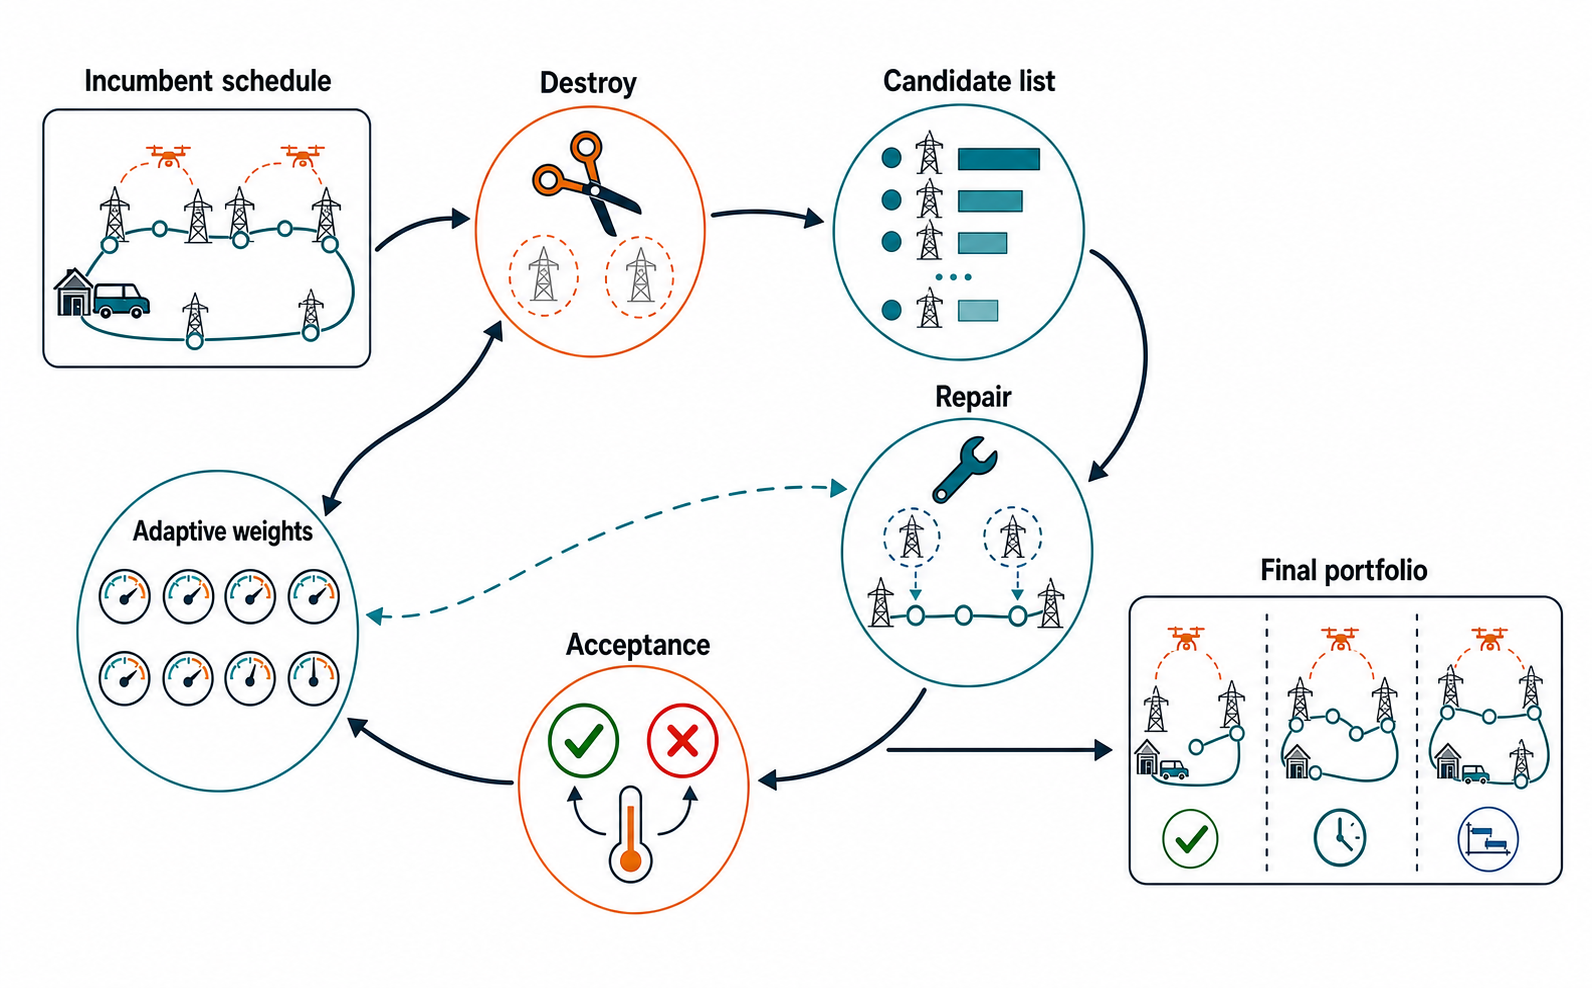
\includegraphics[width=\textwidth]{figures/Fig3_operator_mechanism_ai.png}
\caption{\rev{Adaptive destroy--repair operator mechanism in the energy-surrogate ALNS. The schematic links incumbent schedule disruption, candidate-list construction, greedy/regret/energy/synchronization-aware insertion, simulated-annealing acceptance and adaptive operator scoring.}}
\label{fig:operator-mechanism}
\end{figure*}

\begin{algorithm}[t]
\caption{energy-surrogate ALNS for vehicle--UAV inspection scheduling}
\label{alg:alns}
\begin{algorithmic}[1]
\State Generate candidate stops from corridor clusters.
\State Use the energy surrogate to update $\hat E_i$, $\hat t_i^{air}$, $\hat s_i$ and $\hat B_d$.
\State Build an initial schedule using energy-feasible same-stop sortie patterns.
\State \rev{Initialize deterministic point, UQ and risk-value component orders for the final portfolio.}
\For{$iter=1,\ldots,N_{max}$}
    \State Select destroy and repair operators by adaptive weights.
    \State Remove tasks/stops by random, worst-energy, Shaw, UAV-chain or path-segment destruction.
    \State Repair by greedy insertion, regret-$k$ insertion, energy-minimum insertion or synchronization-aware workload-balancing insertion.
    \State Check endurance feasibility using point or q95 energy surrogate energy.
    \State Accept improving moves; otherwise apply simulated-annealing acceptance.
    \State Update operator scores and weights every $\Delta$ iterations.
\EndFor
\State \rev{Schedule the ALNS-best order and the component orders with the same same-stop launch--recovery scheduler.}
\State \rev{\Return the candidate with the lexicographically best $(\#\mathrm{infeasible},\mathrm{RWCT},C_{max})$.}
\end{algorithmic}
\end{algorithm}

The implemented destroy pool contains random removal, worst-energy removal, Shaw related removal, path-segment removal and UAV-chain removal. The repair pool contains greedy insertion, regret insertion, energy-minimum insertion and synchronization-aware workload-balancing insertion. \rev{Operator use counts, acceptance counts, portfolio candidate counts and selected-candidate diagnostics are exported with the experiment CSV files so that the search behavior can be audited alongside solution quality.}

\paragraph{Computational complexity.}
\rev{Let $n$ be the number of towers, $m$ the number of candidate stops, $I$ the ALNS iteration budget and $q$ the number of removed towers per iteration. Candidate support screening evaluates $O(nm)$ energy estimates, after which clustering reduces the active support layer. Bounded pattern construction groups nearby towers into retained same-stop sortie candidates. With cached tower scores and energy/workload estimates, each ALNS iteration evaluates one destroy--repair move in $O(q+n)$ time for the implemented cached repairs. The final portfolio evaluates a constant number of scheduled orders, so it adds only a constant multiple of the scheduler cost. Under the implemented fixed maximum sortie length, the dominant cost is $O(nm+I(q+n))$ plus the one-time candidate-stop clustering cost.}

For the probabilistic variant, the energy-surrogate interface returns $\mu_E(x_{sk})$ and $\sigma_E(x_{sk})$ for a same-stop pattern $k$ launched from stop $s$. A sortie is accepted only if
\begin{equation}
\mu_E(x_{sk})+z_\epsilon\sigma_E(x_{sk})\leq B_d(1-\rho),
\label{eq:chance}
\end{equation}
where $\rho$ is the reserve ratio. The risk-value objective schedules high-priority towers earlier by using $r_i\nu_i C_i$ in the evaluation layer.

\section{Experimental design}
\label{sec:experiments}

The experiment protocol follows the original design document. Table~\ref{tab:instances} lists the S/M/L instance matrix. Each parameter combination is generated with ten random seeds, giving approximately the same 300--400 instance scale proposed in the initial document once methods and uncertainty levels are counted. \rev{All routing experiments use same-stop launch--recovery sorties; quantile-enabled ALNS variants may group nearby towers into bounded multi-tower sortie patterns, recover the UAV at the launch stop and dispatch it again while the vehicle remains parked.} All raw CSV files, summaries and figure source data are stored under the project experiment folders.

\begin{table*}[t]
\centering
\caption{Proposal-aligned instance scales.}
\label{tab:instances}
\resizebox{\textwidth}{!}{%
\begin{tabular}{@{}lrrrrl@{}}
\toprule
Scale & Towers & Stops & Vehicles & UAVs/vehicle & Use \\
\midrule
S & 10,15,20 & 5,8,10 & 1 & 1--2 & MILP validation\\
M & 30,50,75,100 & 15,25,35,50 & 2--3 & 2--3 & Algorithm comparison\\
L & 150,200,300,500 & 75,100,150,250 & 3--5 & 2--4 & Scalability\\
\bottomrule
\end{tabular}%
}
\end{table*}

The baselines are nearest-neighbor construction, a population-based GA order search, a pheromone-weighted ACO order search, an operator-pool fixed-parameter ALNS baseline, point energy ALNS, uncertainty-aware energy ALNS and the full probabilistic risk-value ALNS. \rev{The proposed row denotes the full probabilistic risk-value ALNS with q95 screening, risk-value ordering, adaptive operator search and metric-aware final portfolio selection.} The GA and ACO baselines report candidate-evaluation diagnostics, while fixed ALNS uses the same destroy--repair operator infrastructure as the proposed method but disables UQ and risk-value weighting. The metrics are makespan, vehicle distance, predicted UAV energy, infeasible sortie rate, risk-weighted completion time, top-risk tower coverage and solver runtime.

\begin{table*}[t]
\centering
\caption{Main simulation and algorithm parameters.}
\label{tab:parameters}
\footnotesize
\begin{tabularx}{\textwidth}{@{}llX@{}}
\toprule
Group & Parameter & Values used in the manuscript experiments \\
\midrule
Instance scale & Towers/stops & S: 10/5, 15/8, 20/10; M: 30/15, 50/25, 75/35, 100/50; L: 150/75, 200/100, 300/150, 500/250. \\
Fleet & Ground vehicles and UAVs & Proposal-defined vehicles and UAVs per vehicle; P8 tests 2, 4 and 6 UAVs on the M50 setting. \\
Energy safety & Reserve ratio $\rho$ and quantile $z_\epsilon$ & Default $\rho=0.12$ and $z_\epsilon=1.645$; P8 tests $\rho\in\{0.08,0.12,0.20\}$ and $z_\epsilon\in\{1.28,1.645,1.96\}$. \\
ALNS & Iteration budget & S: 80, M: 100, L: 60, case: 80; P8 tests 50, 100 and 160 iterations. \\
Candidate stops & Stop generation modes & Direct proposal stops, K-means clustered stops and DBSCAN-style density stops. \\
Replication & Random seeds & Ten seeds for P1--P4, P6 and P8; five seeds for the realistic case study; P7 uses paired tests over P2 summaries. \\
\bottomrule
\end{tabularx}
\end{table*}

\begin{figure*}[t]
\centering
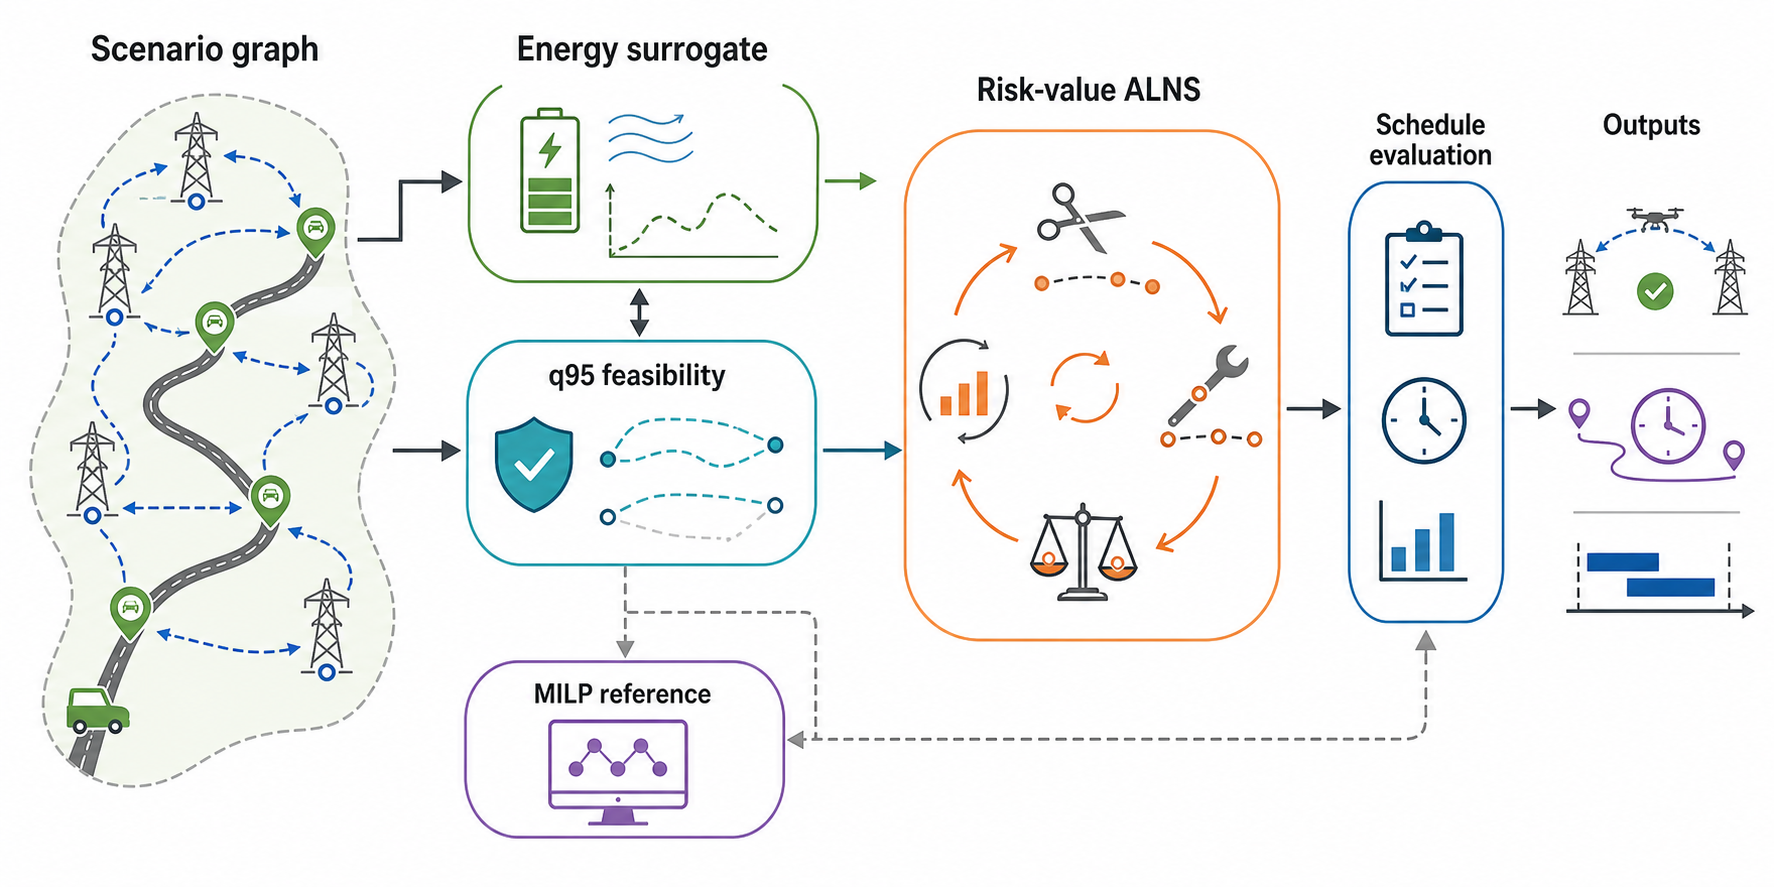
\includegraphics[width=\textwidth]{figures/Fig1_framework_ai.png}
\caption{MILP--energy-surrogate--ALNS workflow aligned with the original research proposal.}
\label{fig:framework}
\end{figure*}

\begin{figure*}[t]
\centering
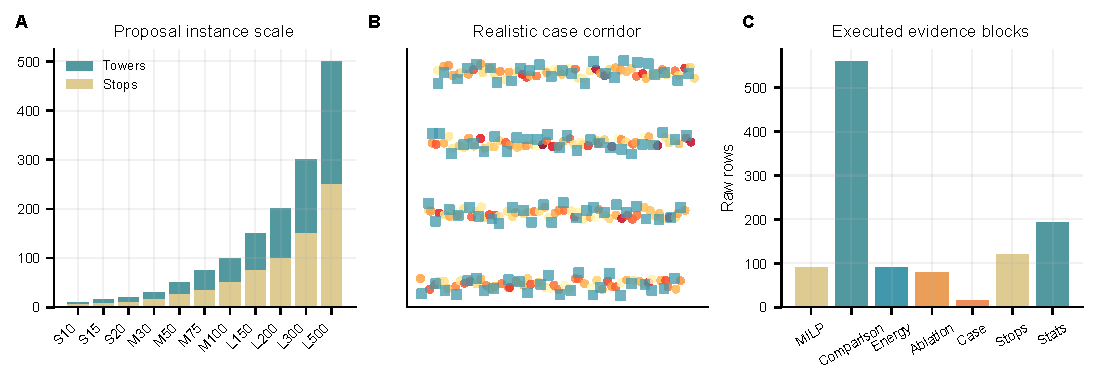
\includegraphics[width=\textwidth]{figures/Fig2_instances.pdf}
\caption{Proposal-defined S/M/L instance design, realistic corridor case and executed evidence blocks.}
\label{fig:instances}
\end{figure*}

\section{Results}
\label{sec:results}

\subsection{Small-scale MILP validation}

Figure~\ref{fig:milp} reports the S-scale validation block. The average proposed ALNS gap to the compact MILP reference across S instances is 45.19\% under the makespan comparison used in the experiment table. The compact reference is used as a bounded small-instance sanity check rather than as a complete exact RWCT benchmark. This is consistent with the role specified in the proposal: compact reference optimization is used for S-scale validation, while energy ALNS is used for scalable solution.

\begin{figure*}[t]
\centering
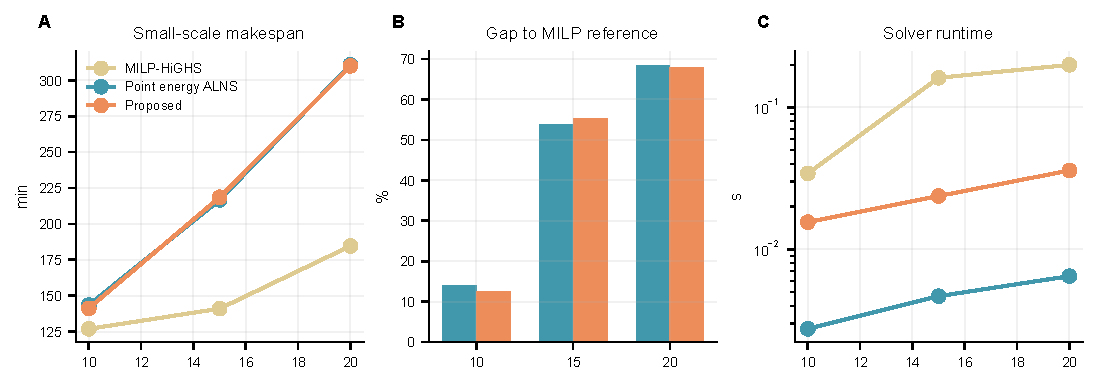
\includegraphics[width=\textwidth]{figures/Fig3_milp_validation.pdf}
\caption{Small-scale MILP/HiGHS validation: makespan, gap to reference and runtime.}
\label{fig:milp}
\end{figure*}

\subsection{Algorithm comparison}

Figure~\ref{fig:comparison} compares algorithms on the 100-tower benchmark. \rev{Across the matched 30--500 tower benchmarks, the proposed method reduces mean RWCT relative to fixed ALNS by 40.44\%--46.10\%. It also improves mean RWCT over point energy ALNS by 0.27\%--4.30\% and over UQ energy ALNS by 1.16\%--4.17\%.} The paired RWCT comparison against point energy ALNS has a median effect of 1.9 risk-time units and a Holm-adjusted Wilcoxon value of $p_{Holm}=0.0560$ at 100 towers. Top-risk coverage is also interpreted after the same correction, with $p_{Holm}=0.952$. \rev{The q95 feasibility layer reduces the infeasible-sortie rate from 0.20\% to 0.00\% on the same benchmark, indicating that the risk-value and uncertainty layers improve both schedule priority and sortie feasibility.}

\begin{figure*}[t]
\centering
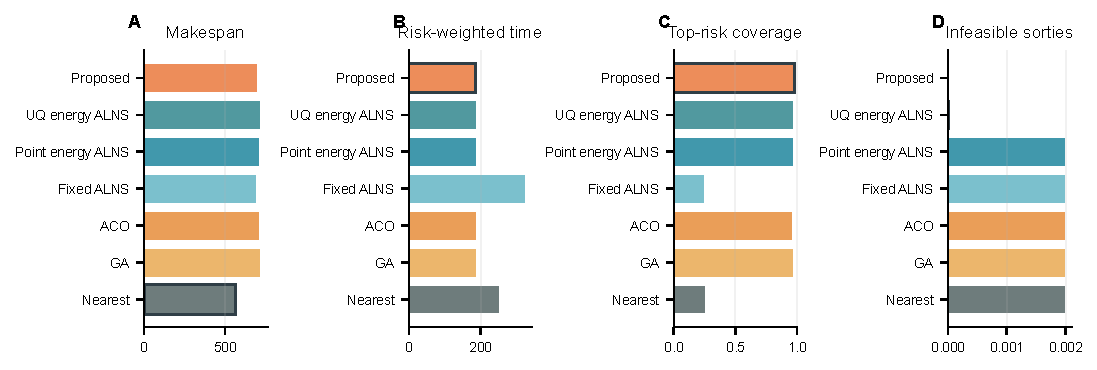
\includegraphics[width=\textwidth]{figures/Fig4_algorithm_comparison.pdf}
\caption{Algorithm comparison on the 100-tower benchmark.}
\label{fig:comparison}
\end{figure*}

\subsection{Energy prediction validation}

Figure~\ref{fig:energy-surrogate} evaluates fixed physics, point prediction and the simulation-trained probabilistic residual surrogate. The surrogate is trained on 936 synthetic physics-residual samples and evaluated on held-out scenario seeds. Under high uncertainty, the probabilistic surrogate obtains a 95\% interval coverage of 100.0\%, compared with 43.0\% for point prediction and 10.2\% for fixed physics. It also reduces high-uncertainty MAE from 12.96 and 9.40 energy units for the two baselines to 1.30. \rev{The calibrated interval gives the scheduler a direct q95 feasibility screen for same-stop sortie patterns.}

\begin{figure*}[t]
\centering
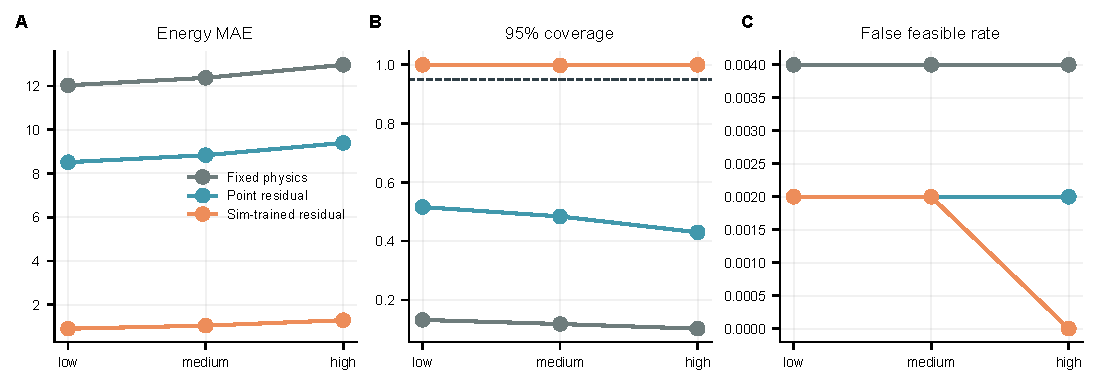
\includegraphics[width=\textwidth]{figures/Fig5_energy_surrogate_accuracy.pdf}
\caption{\rev{Energy prediction validation with residual-surrogate labels: energy error, interval coverage and false-feasible rate.}}
\label{fig:energy-surrogate}
\end{figure*}

\subsection{Ablation and case study}

Figure~\ref{fig:ablation} shows that removing the energy surrogate, adaptive search, uncertainty filter, risk-value term, repair operators or clustering stage weakens at least one of the paper's target outcomes. The no-surrogate variant has poor high-risk coverage, removing the risk-value term reduces high-risk coverage, and removing clustering worsens the risk-time objective despite retaining feasibility. The repair-specific ablation indicates a search-dynamics contribution: disabling energy-minimum or synchronization-aware repair leaves the current M50 aggregate risk-time nearly unchanged, but reduces improving ALNS moves by 4.6\% and 35.6\%, respectively. Figure~\ref{fig:case} reports the realistic 200-tower corridor case. The proposed ALNS reduces risk-weighted completion time by 43.7\% compared with fixed ALNS and increases top-risk coverage by 76.0 percentage points.

\begin{figure*}[t]
\centering
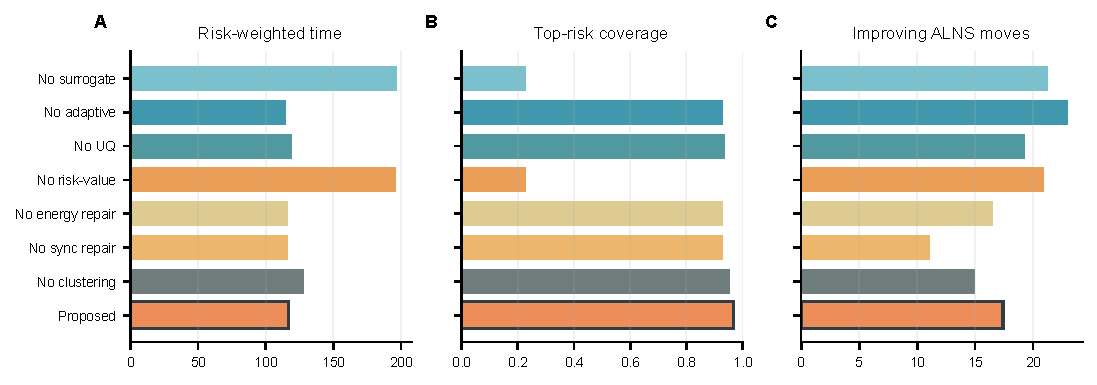
\includegraphics[width=\textwidth]{figures/Fig6_ablation.pdf}
\caption{Ablation results for energy surrogate, adaptive search, uncertainty, risk-value and clustering components.}
\label{fig:ablation}
\end{figure*}

\begin{figure*}[t]
\centering
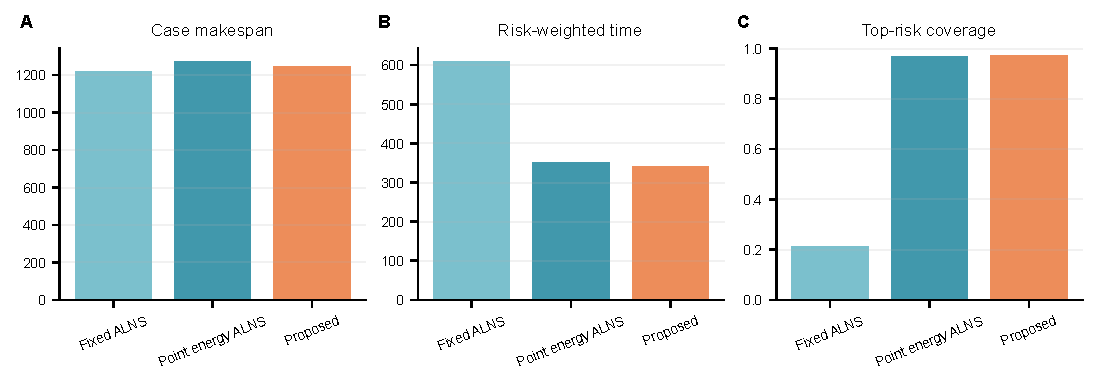
\includegraphics[width=\textwidth]{figures/Fig7_case_study.pdf}
\caption{Realistic corridor case study with 200 towers and 100 candidate stops.}
\label{fig:case}
\end{figure*}

\subsection{Scalability}

Figure~\ref{fig:scalability} reports S/M/L scalability from 30 to 500 towers. \rev{At 500 towers, the proposed method reduces mean RWCT by 42.0\% relative to fixed ALNS and by 1.71\% relative to point energy ALNS.} Against the point variant, the paired RWCT effect is 5 risk-time units with $p_{Holm}=0.3229$, and top-risk coverage has $p_{Holm}=0.9519$. Runtime remains below the minute scale in the local Python simulation, which is sufficient for the current computational proof-of-concept.

\begin{figure*}[t]
\centering
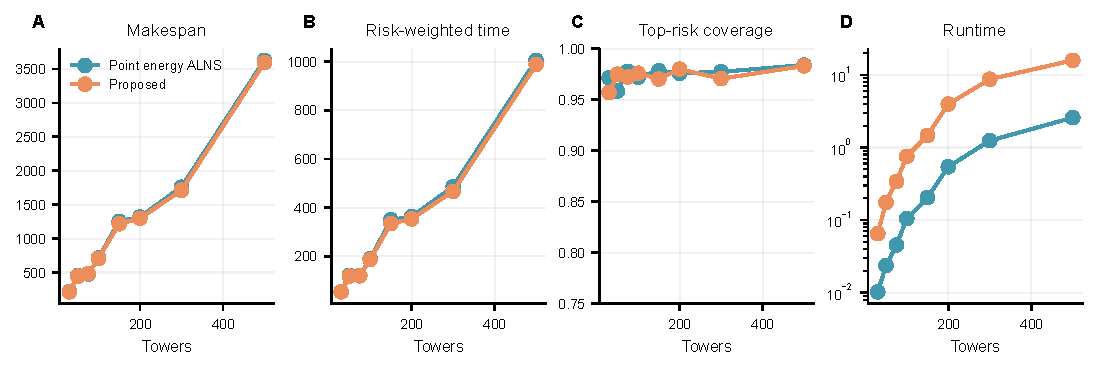
\includegraphics[width=\textwidth]{figures/Fig8_scalability.pdf}
\caption{Scalability from 30 to 500 towers.}
\label{fig:scalability}
\end{figure*}

\subsection{Candidate-stop screening and statistical evidence}

Figure~\ref{fig:screening} reports the candidate-stop screening and statistical evidence block. K-means candidate-stop generation reduces screened service candidates by 94.0\% on 100-tower instances, whereas DBSCAN reduces the candidate count by 58.1\% but produces worse makespan in this corridor generator. This supports using deterministic K-means as the default candidate-stop generator in the simulation experiments. The right panels of Fig.~\ref{fig:screening} summarize the paired statistical tests: the strongest evidence is for risk-weighted completion time rather than nominal makespan.

\begin{figure*}[t]
\centering
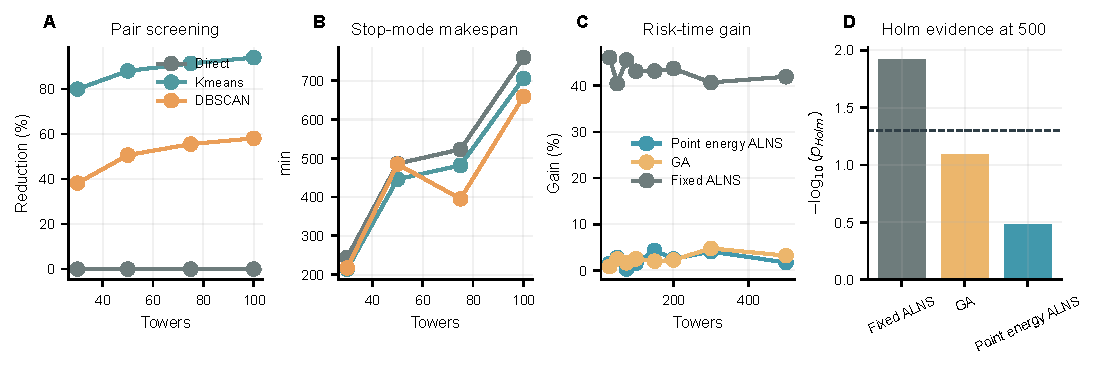
\includegraphics[width=\textwidth]{figures/Fig9_candidate_screening_statistics.pdf}
\caption{Candidate-stop screening and paired statistical evidence.}
\label{fig:screening}
\end{figure*}

\subsection{Parameter sensitivity}

Figure~\ref{fig:sensitivity} summarizes the sensitivity batch for candidate-stop mode, UAV count, iteration budget, quantile coefficient and reserve ratio. In this M50 high-uncertainty setting, K-means reduces risk-weighted completion time by 9.8\% relative to direct stop enumeration while retaining zero infeasible sorties; DBSCAN is less reliable and has a 71.8\% infeasible-sortie rate after screening. Increasing the UAV count from four to six reduces makespan by 0.0\%, whereas using only two UAVs increases makespan substantially. Raising the ALNS iteration budget mainly increases improving moves by 43.1\% rather than changing aggregate risk-time, suggesting that the current objective landscape is already stable on the M50 batch.

\begin{figure*}[t]
\centering
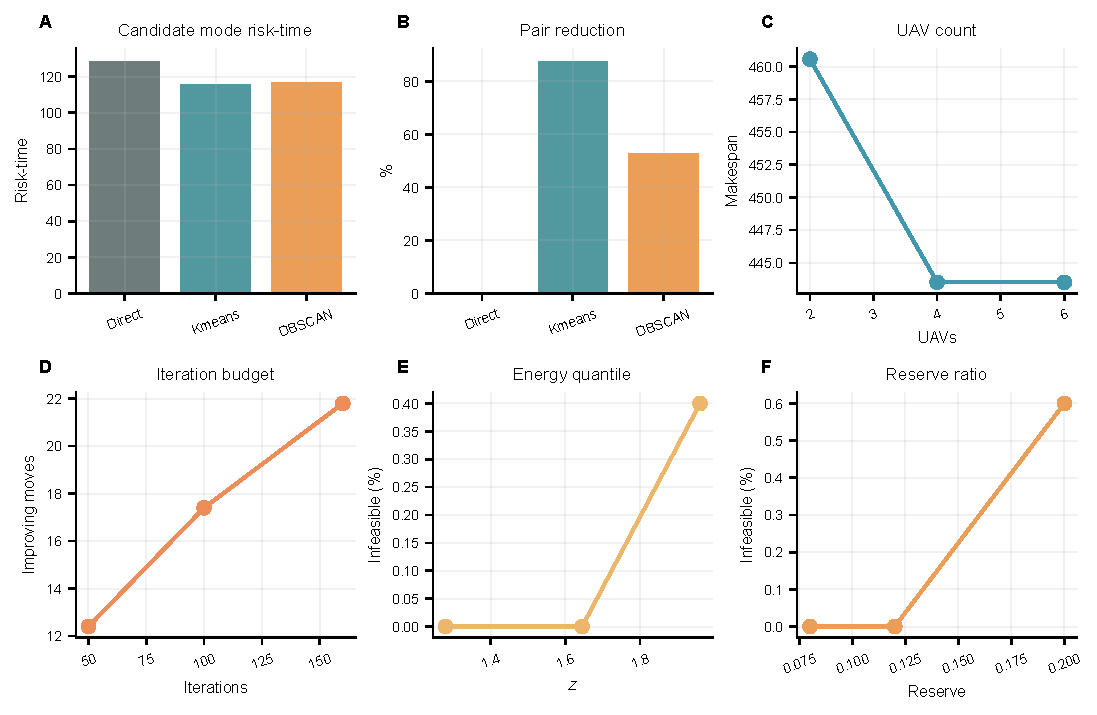
\includegraphics[width=\textwidth]{figures/Fig10_sensitivity.pdf}
\caption{Sensitivity analysis for candidate-stop mode, fleet size, search budget and energy-safety parameters.}
\label{fig:sensitivity}
\end{figure*}

\clearpage

\section{Discussion}
\label{sec:discussion}

\rev{The computational evidence shows that the proposed method is most useful when inspection priority and energy safety are evaluated together. The main effect is the combined improvement in high-risk task coverage, q95 energy-feasibility screening and large-scale solvability. This matches the operational nature of transmission-line inspection, where early inspection of high-risk towers and avoidance of unsafe sorties can be more important than nominal travel-time reduction alone.}

\rev{The evidence also has clear boundaries. The routing data are simulated corridor instances and public GIS-grounded proxy cases, the compact MILP reference is limited to S-scale validation, and the residual energy surrogate is trained on synthetic physics-residual labels with public telemetry used as a separate calibration check. Stress tests show that conservative uncertainty handling improves infeasible-sortie rates and top-risk coverage, while some no-UQ cases can produce lower RWCT under adverse settings. These boundaries limit deployment claims and motivate real inspection-log calibration.}

\section{Conclusion}
\label{sec:conclusion}

\rev{This paper formulates vehicle--UAV cooperative transmission-line inspection scheduling with same-stop multi-tower sortie patterns, explicit energy and endurance parameters, repeated UAV dispatch after recovery and parallel UAV operation at a parked vehicle stop.} It checks small instances with a compact MILP reference and evaluates an uncertainty-aware ALNS across S/M/L instances up to 500 towers. \rev{The full probabilistic risk-value variant reduces mean RWCT by 40.4\%--46.1\% relative to fixed ALNS across the tested 30--500 tower scales and protects sortie feasibility through q95 energy screening.} K-means candidate-stop generation substantially reduces support-candidate enumeration while the scheduler evaluates bounded same-stop sortie patterns in the tested corridor instances. \rev{Future work should couple the scheduler with online re-dispatch, dynamic wind and road-state updates, real utility inspection logs, defect labels and field battery records.}

\section*{CRediT authorship contribution statement}
To be completed by the authors.

\section*{Declaration of competing interest}
The authors declare that they have no known competing financial interests or personal relationships that could have appeared to influence the work reported in this paper.

\section*{Data availability}
The current manuscript uses synthetic simulation data generated by the project scripts. Raw CSV files, summary tables, figure source data and LaTeX sources are stored in the local project directory.

\bibliography{tre_references}

\end{document}
